\documentclass[a4paper, 14pt]{article}
\usepackage[dvipsnames]{xcolor}
\usepackage[top=70pt,bottom=70pt,left=48pt,right=46pt]{geometry}
\definecolor{header}{RGB}{92,184,92}
\definecolor{defenition}{RGB}{217,83,79}
\definecolor{main_title}{RGB}{66,139,202}
\definecolor{sub_header}{RGB}{91,192,222}
\usepackage[english, russian]{babel}
\usepackage[utf8]{inputenc}
\usepackage{amsmath}
\usepackage{listings}
\usepackage{graphicx}
\usepackage{amsmath}
\title{\textcolor{main_title}{Исследование фотопроводимости полупроводников}}
\author{Шмаков Владимир Евгеньевич - ФФКЭ гр. Б04-105}






\begin{document}
\maketitle

\section*{\textcolor{header}{Цель работы}}

\begin{enumerate}
    \item Познакомиться с явлением фотопроводимости
    \item Оценить ширину запрещенной зоны CdS и CdSe
\end{enumerate}

\section*{\textcolor{header}{Теоретические сведения}}

	
Электропроводность полупроводника увеличивается под действием света. 
Это явление называется \textcolor{defenition}{\textbf{фотопроводимостью}} или {внутренним фотоэффектом}. 

В отсутствии света в полупроводнике присутствует некоторое количество носителей тока: электроны переходя из валентной зоны в зону проводимости (в случае наличия примесей возможны также переходы с донорных на акцепторные уровни) в результате теплового движения. Количество таких носителей определяется температурой кристалла, они называются равновесными и составляют темновой ток. 

Фотопроводимость проявляется в случае, если энергия квантов превышает некоторое пороговое значение. Для собственной фотопроводимости это значение равно ширине запрещенной зоны, а в случае примесной --- энергии ионизации соответствующего уровня. Минимальная частота света, при которой возможно появление неравновесных электронов (то есть, электронов фотопроводимости), называется красной границей фотоэффекта. При этом можно считать, что включение света не влияет на концентрацию равновесных электронов. 








\section*{\textcolor{header}{Методика}}
\subsection*{\textcolor{sub_header}{Оборудование}}

\begin{itemize}
    \item Призменный монохроматор 
    \item Лампа накаливания 
    \item Неоновая Лампа - для проверки градуировки
    \item Набор линз 
    \item Вольтметр
    \item Исследуемые образцы 
\end{itemize}

\subsection*{\textcolor{sub_header}{Экспериментальная установка}}

В работе исследуются два образца: CdS и CdSe. 
Схема установки приведена на рисунке \ref{pic:scheme}. 
Свет от источника И с помощью линзы Л фокусируется на щель монохроматора УМ-2, 
находящуюся в фокусе линзы Л$_1$. Пучое света разлагается призмой П, и выходная щель, находящаяся в фокусе линзы Л$_2$, вырезает отпределенную область спектра. После прохождения монохроматора свет падает на ячейку Я с образцом. Вольтметр В7-34 нужен для измерения тока через образец. 

\begin{figure}[h]

    \centering	
    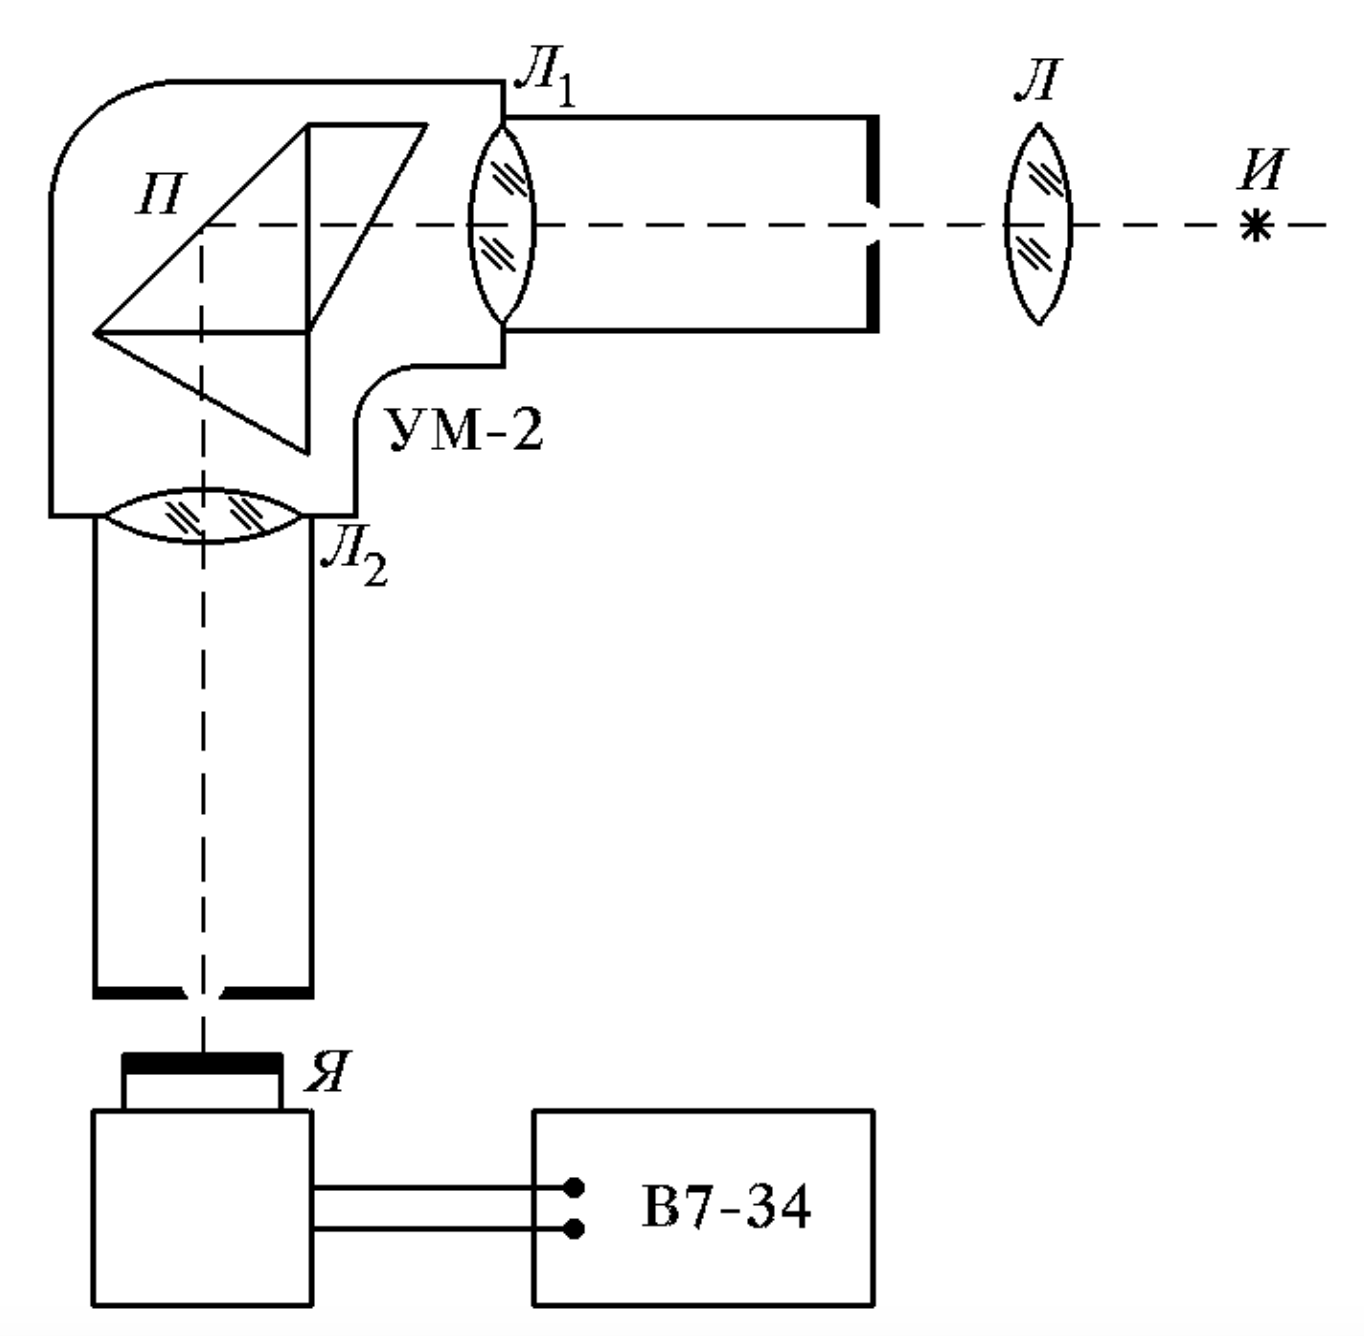
\includegraphics[width=0.4\textwidth]{lab.png}
    \caption{Схема экспериментальной установки}
    \label{pic:scheme}
\end{figure} 

Для корректировки градуировки монохроматора используется неоновая лампа. В спектре неона несложно найти 
желтый дуплет. Ориентируясь на дуплет можно проверить корректность градуировочных кривых.


\section*{\textcolor{header}{Обработка экспериментальных данных}}


\subsection*{\textcolor{sub_header}{Градуировочные кривые}}

Для дальнейшей обработки экспериментальных данных потребуются градуировочные кривые.
Как видно на рисунке $\ref{fig:grad}$, обе градуировочные кривые хорошо приближаются 
экспоненциальной функцией вида $a e^{c(x - b)} + d$.

\begin{figure}[htbp]
    \centering
    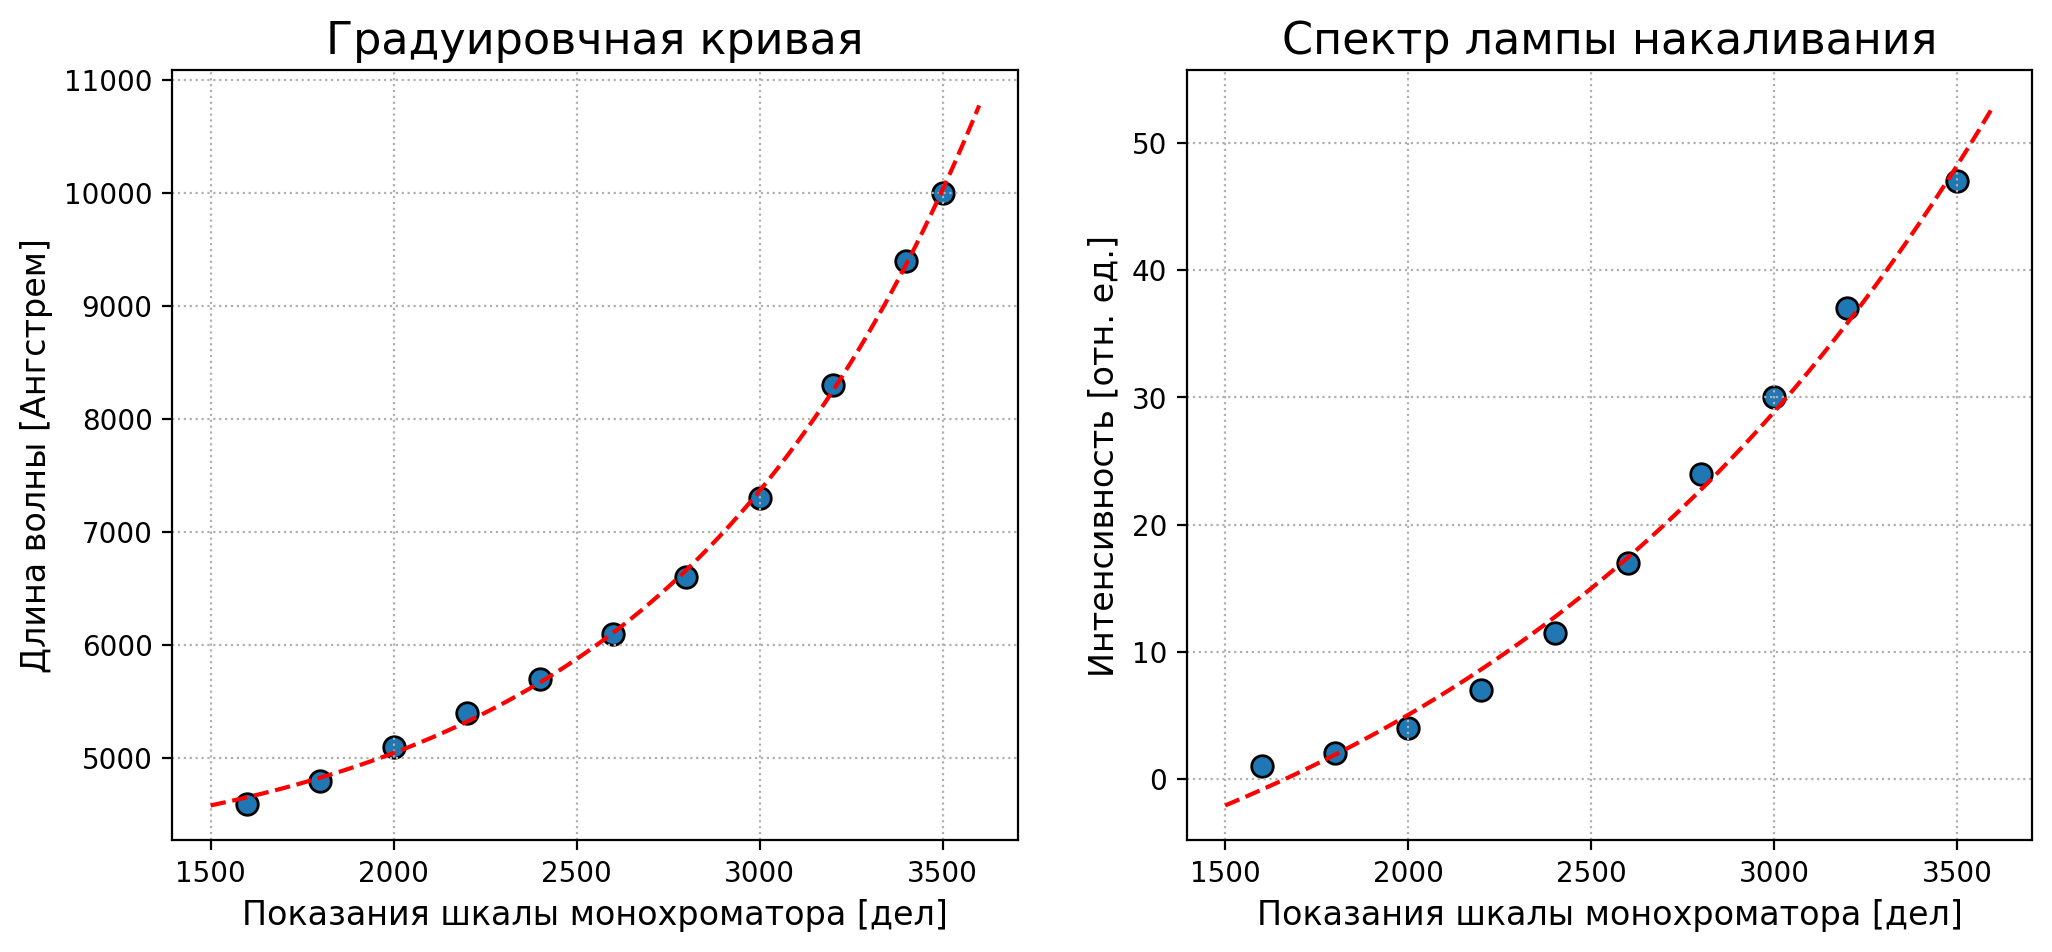
\includegraphics[width=0.9\textwidth]{grad.png}

    \caption{Приближение градуировочных кривых экспоненциальной функцией}
    \label{fig:grad}
\end{figure}




\subsection*{\textcolor{sub_header}{CdSe}}

Для построения зависимости \textcolor{defenition}{фотоответа} - количества электронов на
один упавший фотон от длины волны используется следующий алгоритм:
\begin{itemize}
    \item По градуировочной кривой зависимости длины волны от показаний монохроматора переводим ось $x$ в ангстремы.
    \item Для вычисления фотоответа делим экпериментально полученное значения напряжения на интенсивность при данном значении шкалы.
\end{itemize}

Построим зависимость фотоответа от длины волны для образца Кадмий-Селена.
\begin{figure}[htbp]
    \centering
    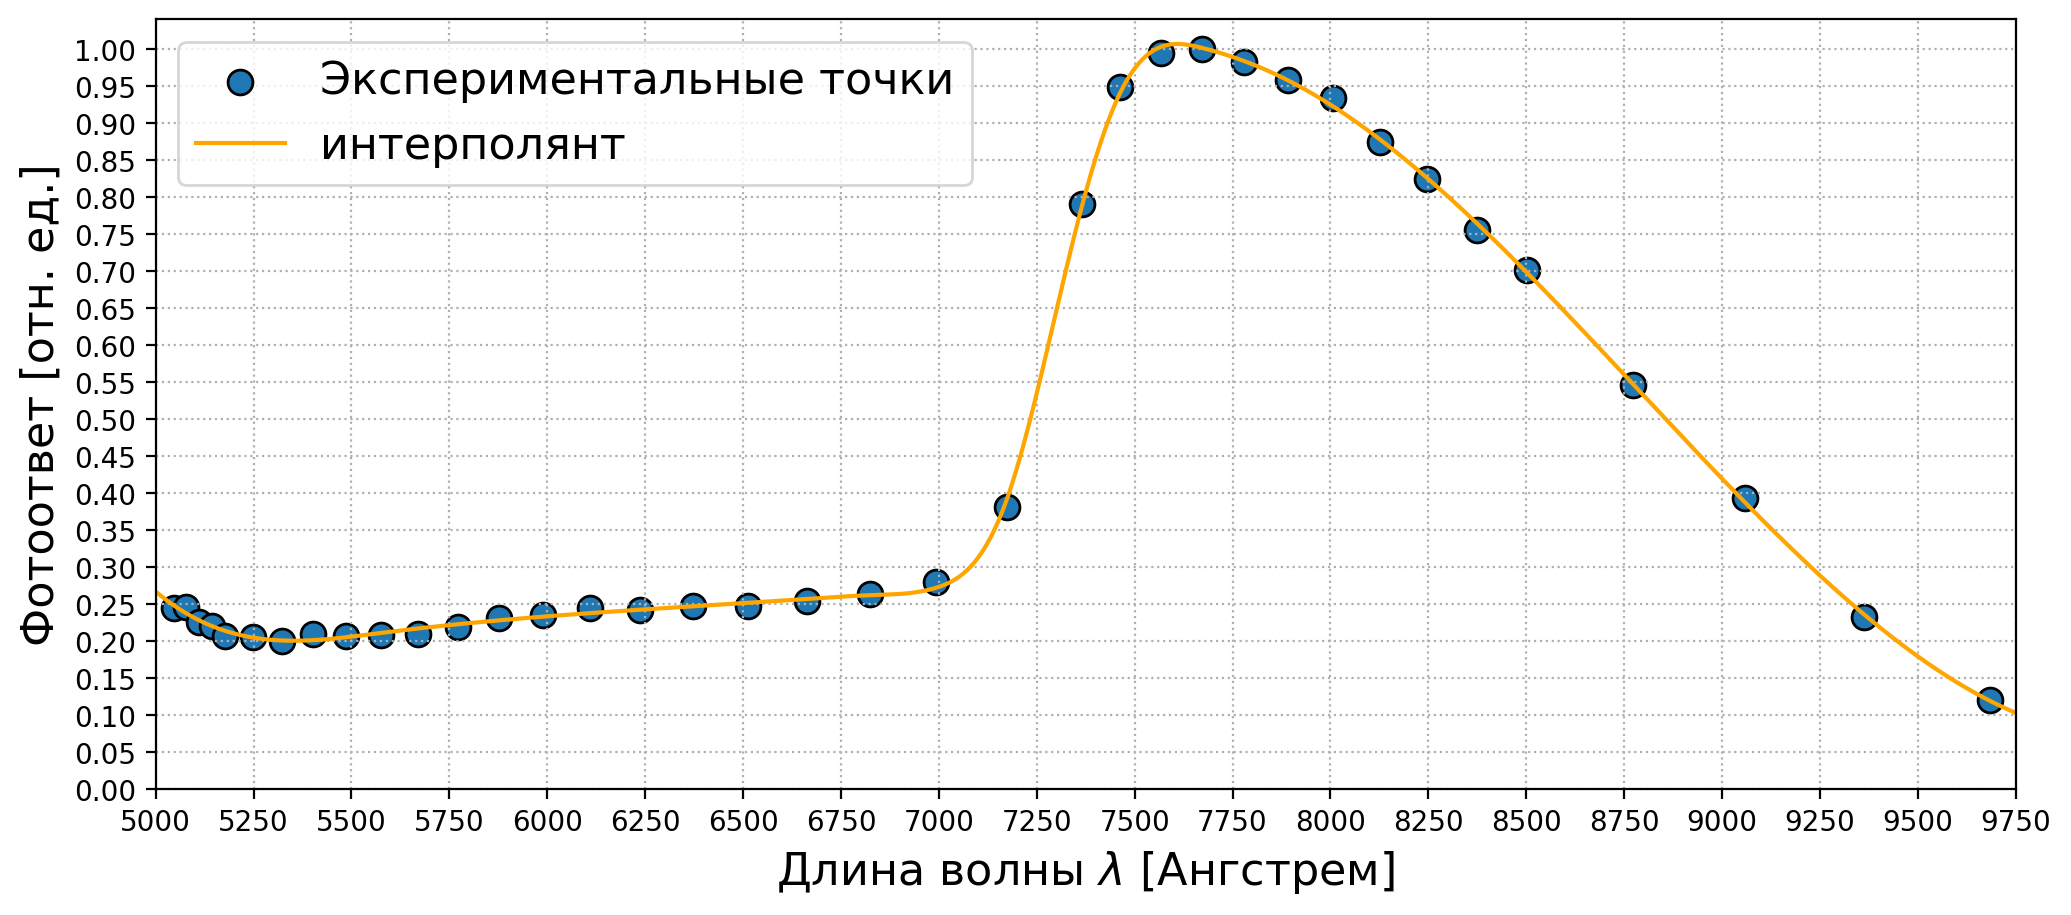
\includegraphics[width = 0.9\textwidth]{CdSe_main.png}
    \caption{Спектральная зависимость для образца CdSe}
    \label{fig:CdSe_main}
\end{figure}

Для нахождения ширины запрещенной зоны оценим красную границу эффекта как велину $\lambda$ при
которой фотоответ падает в два раза. Тогда $\lambda_{CdSe}^{кр} \sim 875 \text{ нм}$, что соответствует
энергии $E_{CdSe} = 1.417 \text{ эВ}$.

Для лучшей оценки следует построить зависимость фотоответа от энергии. Для прямозонных полупроводников
зависимость квадрата фотоответа от энергии имеет линейный характер. Пересечение наилучшей прямой с осью
энергий даёт ширину запрещенной зоны.

\subsection*{\textcolor{sub_header}{CdS}}

\begin{figure}[htbp]
    \centering
    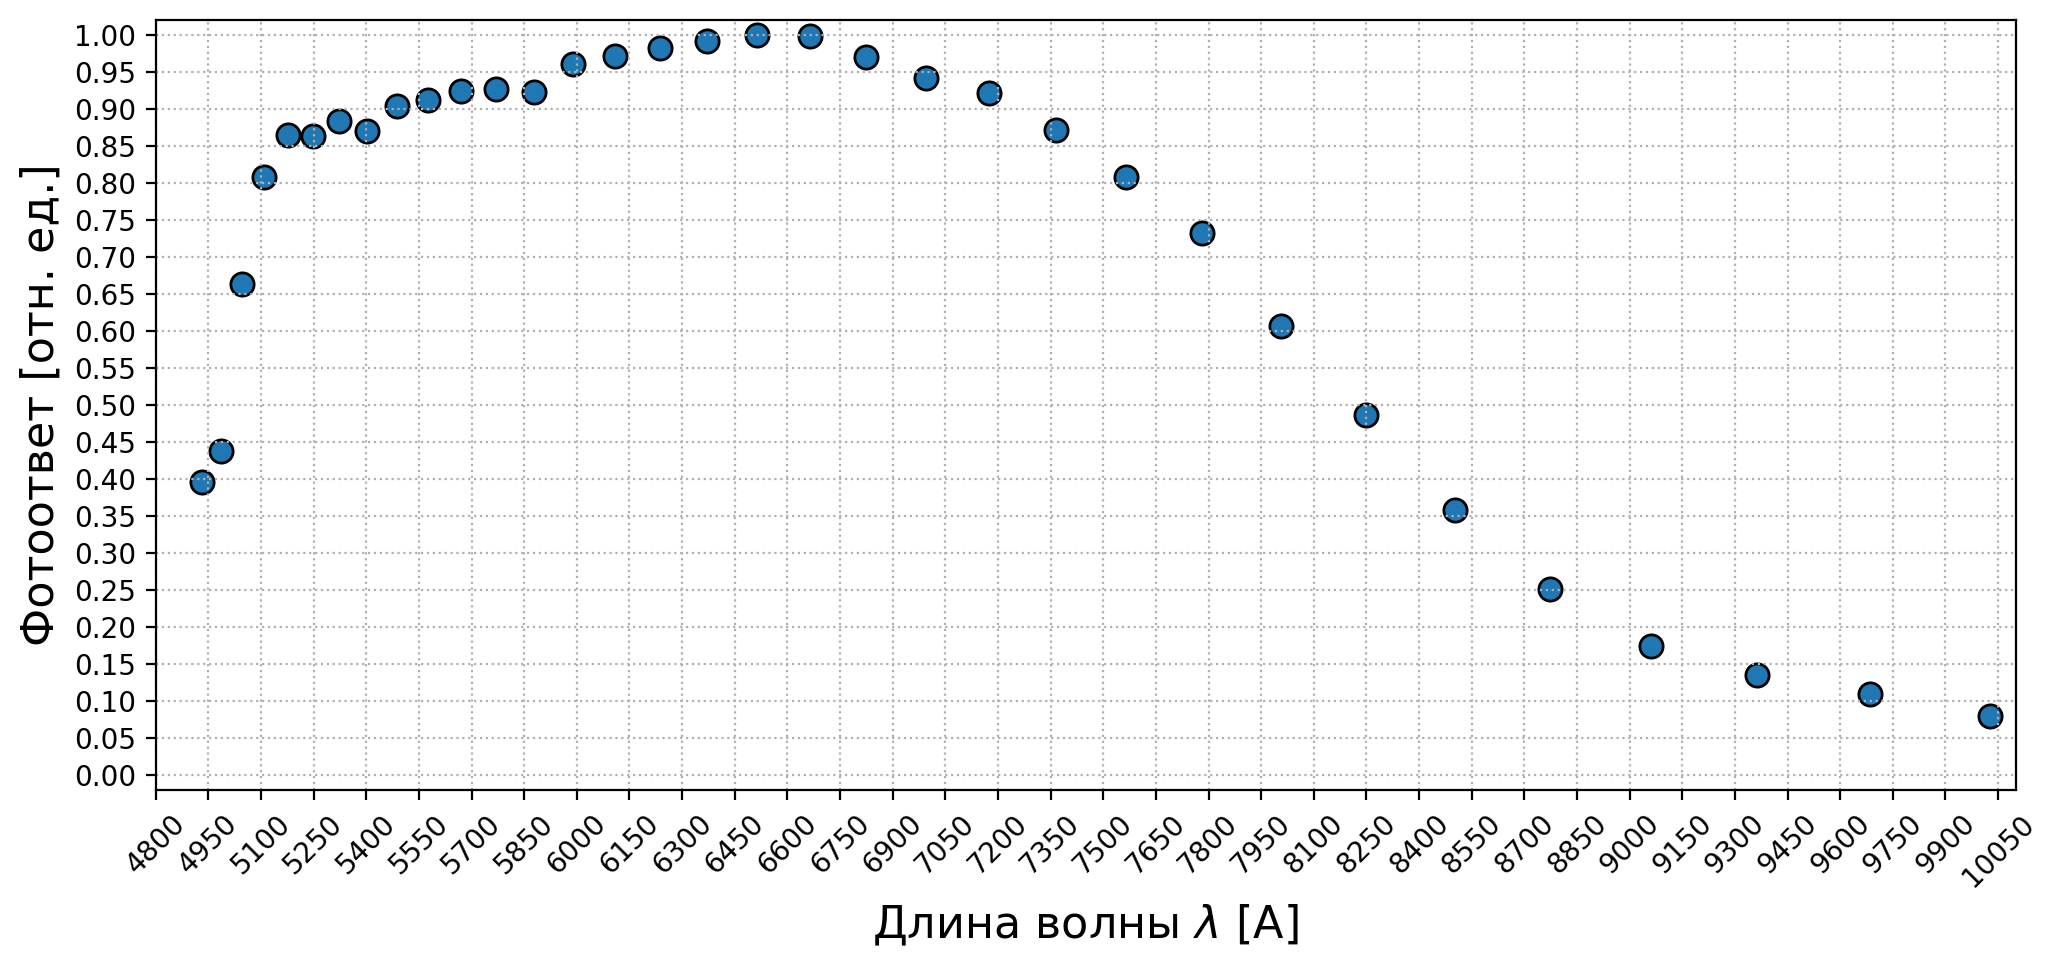
\includegraphics[width = 0.8 \textwidth]{CdS_main.png}
    
    \caption{Спектральная зависимость для образца CdS}
    \label{fig:CdS_main}
\end{figure}

Аналогично для $CdS$: $\lambda_{кр} = 740 \text{нм}$, что соответствует энергии 
$E_{CdS} = 1.7 \text{ Эв}$


\section*{\textcolor{header}{Вывод}}

Удалось оценить ширину запрещенной зоны двух образцов. Погрешность измерения 
оказалсь достаточно большой. 

Ошибка может быть связана с двумя факторами:
\begin{enumerate}
    \item Неверная <<умозрительная>> методика оценки $\lambda_{кр}$.
    \item Невереная градуировка монохроматора.
\end{enumerate}





\end{document}
